\documentclass[border=10pt]{standalone}

\usepackage{tikz}
\usepackage{tikzsymbols}
\usetikzlibrary{calc,patterns,shapes.geometric}

\def\centerarc[#1](#2)(#3:#4:#5){\draw[#1] ($(#2)+({#5*cos(#3)},{#5*sin(#3)})$) arc (#3:#4:#5);}

\begin{document}
	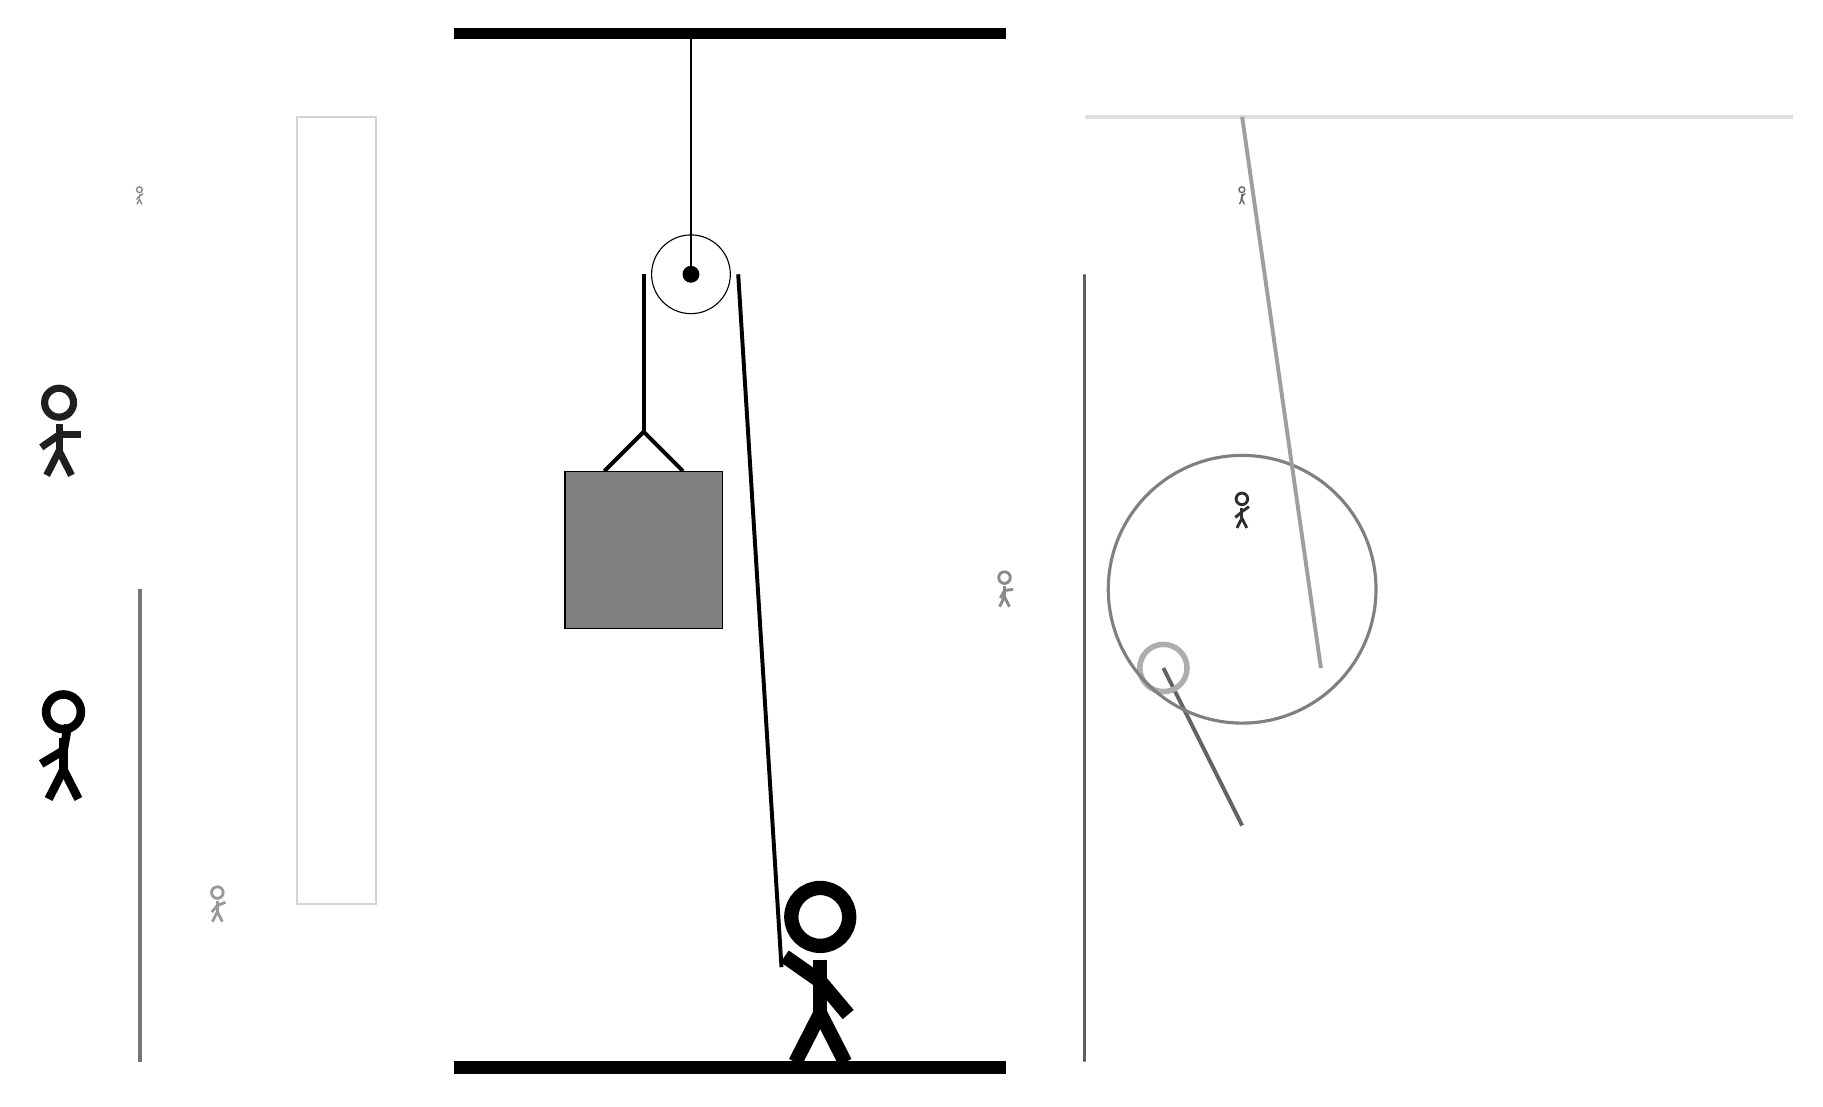
\begin{tikzpicture}
		%%%%% START %%%%%
		
		\draw[fill=black] (-2, 10) rectangle (5, 10.125);
		
		\draw (1, 7) circle (0.5);
		\draw[fill=black] (1, 7) circle (0.1);
		\draw (1, 10) -- (1, 7);
		
		\draw[line width=0.5mm] (-0.1, 4.5) -- (0.4, 5.0) -- (0.9, 4.5);
		\draw[fill=black!50] (-0.6, 4.5) rectangle (1.4, 2.5);
		
		\node[line width=0.4mm, color=black!100] at (-7, 1) {\Strichmaxerl[6][31][80]};
		
		\draw[line width=0.5mm, color=black!13](6, 9) -- (15, 9);
		\draw[line width=0.5mm, color=black!61](8, 0) -- (7, 2);
		\node[line width=0.5mm, color=black!45] at (-6, 8) {\Strichmaxerl[1][47][33]};
		\draw[line width=0.3mm, color=black!63] (6, -3) rectangle (6, 7);
		\draw [line width=0.3mm, color=black!19](-7, 3) circle (0.0);
		
		\draw [line width=0.7mm, color=black!32](7, 2) circle (0.3);
		\draw[line width=0.5mm, color=black!54](-6, 3) -- (-6, -3);
		\node[line width=0.4mm, color=black!82] at (8, 4) {\Strichmaxerl[2][41][36]};
		\node[line width=0.7mm, color=black!88] at (-7, 5) {\Strichmaxerl[5][35][0]};
		\draw [line width=0.4mm, color=black!50](8, 3) circle (1.7);
		
		\node[line width=0.4mm, color=black!58] at (8, 8) {\Strichmaxerl[1][77][38]};
		\node[line width=0.2mm, color=black!40] at (-5, -1) {\Strichmaxerl[2][50][21]};
		
		\draw[line width=0.3mm, color=black!17] (-4, 9) rectangle (-3, -1);
		\node[line width=0.5mm, color=black!46] at (5, 3) {\Strichmaxerl[2][62][7]};
		\draw[line width=0.5mm, color=black!38](9, 2) -- (8, 9);
		
		
		\draw[line width=0.5mm] (0.4, 7) -- (0.4, 5.0);
		\centerarc[line width=0.5mm](1, 7)(0:180:0.6);
		\draw[line width=0.5mm](1.6, 7) -- (2.15, -1.8);
		
		\node at (2.6, -1.9) {\Strichmaxerl[10][-35][-50]};
		
		\draw[fill=black] (-2, -3) rectangle (5, -3.15);
		
		%%%%% END %%%%%
	\end{tikzpicture}
\end{document}